\section{WINDOWS软硬件系统观察与分析}
\subsection{查看计算机基本信息(2分)}

截图:
\begin{itemize}
	\item 控制面板->系统
	\item 命令行systeminfo执行结果(至少包含启动设备行)
\end{itemize}

\begin{figure}[H]
	\begin{minipage}[c]{0.58\linewidth}
		\centering
		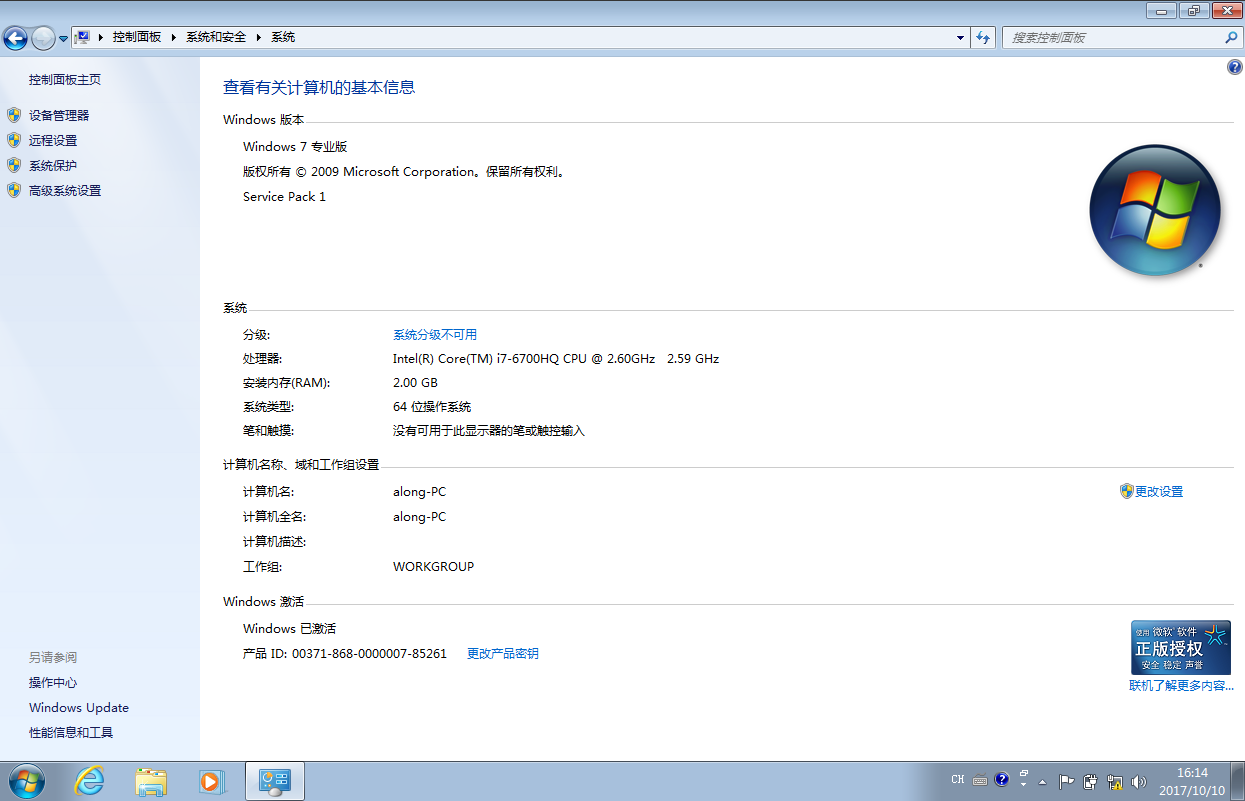
\includegraphics[width=\linewidth]{figures/Win-Ctl-System}
		\label{fig:win-ctl-system}
	\end{minipage}
	\begin{minipage}[c]{0.3\linewidth}
		\centering
		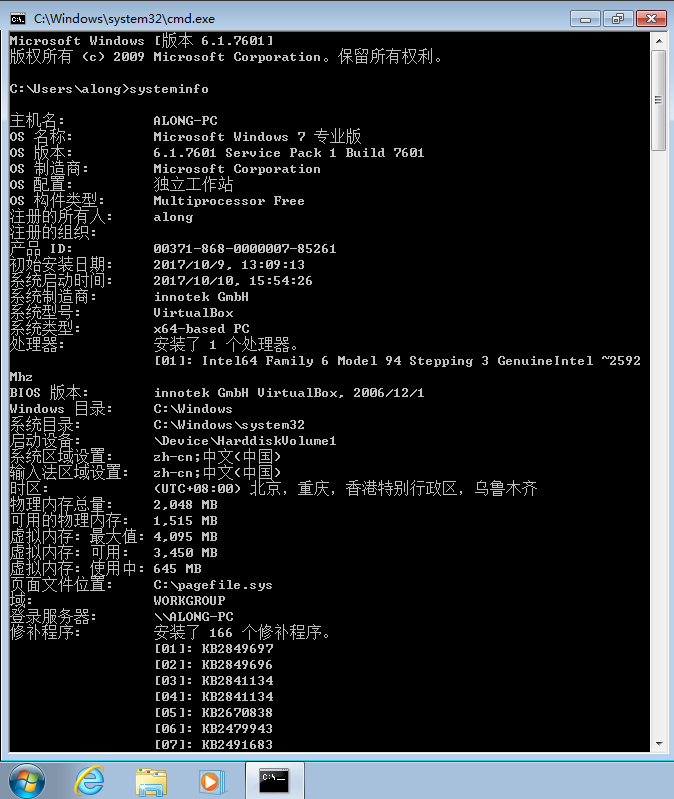
\includegraphics[width=\linewidth]{figures/Win-SysInfo}
		\label{fig:win-sysinfo}
	\end{minipage}
	\caption{Windows下计算机基本信息}
\end{figure}

\subsection{设备管理器查看(2分)}
按链接列出设备,找出所有的键盘鼠标设备。写出每一个设备的从根到叶节点的路径。

\begin{itemize}
	\item 键盘:along-PC/键盘/PS/2标准键盘
	\item 鼠标1:along-PC/鼠标和其他指针设备/HID-compliant mouse
	\item 鼠标2(若有):along-PC/鼠标和其他指针设备/Microsoft PS/2 Mouse
\end{itemize}

\subsection{隐藏分区与虚拟内存之分页文件查看(2分)}

\begin{itemize}
	\item 写出计算机主硬盘的各隐藏分区的大小(MB):100MB
	\item 写出pagefile.sys的文件大小(Byte):2,147,016,704字节
	\item C盘根目录下其他隐藏的系统文件名字为:
		\subitem \$Recycle.Bin
		\subitem Document and Settings
		\subitem ProgramData
		\subitem Recovery
		\subitem System Volume Information
\end{itemize}

\subsection{任务管理与资源监视(2分)}

写出你的计算机的PID最小的两个任务的名称、描述。

\begin{enumerate}
	\item 系统中断 延迟过程调用和中断服务例程
	\item System NT Kernel \& System
\end{enumerate}

\subsection{计算机硬件详细信息(2分)} 

\begin{itemize}
	\item CPU个数:\dlmu[3cm]{1}
	\item 物理核数:\dlmu[3cm]{2}
	\item 逻辑处理器个数:\dlmu[3cm]{2}
	\item L1 Cache大小:\dlmu[3cm]{2x32KBytes}
	\item L2 Cache大小:\dlmu[3cm]{2048KBytes}
\end{itemize}

\begin{figure}[H]
	\centering
	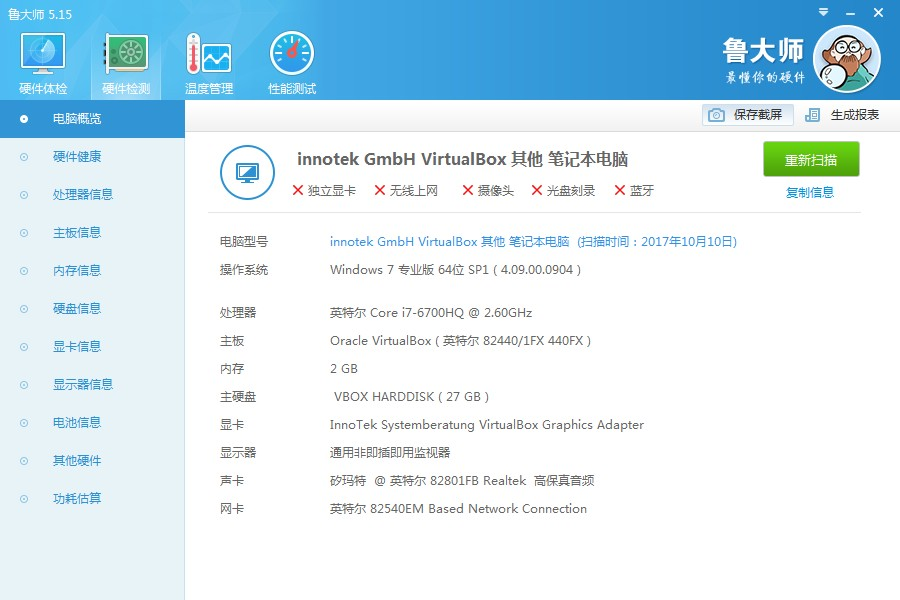
\includegraphics[width=0.7\linewidth]{figures/Win-HarewareInfo}
	\caption{Windows下计算机硬件详细信息}
	\label{fig:win-harewareinfo}
\end{figure}



